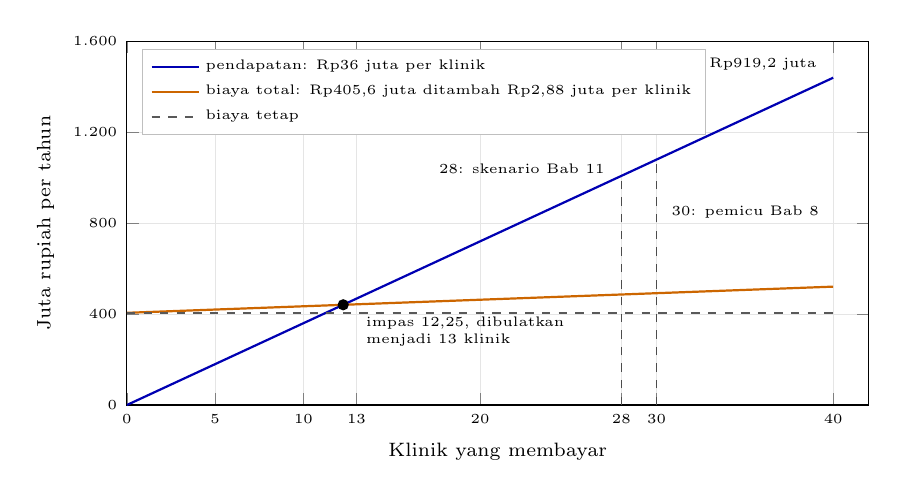
\begin{tikzpicture}[font=\scriptsize]
  \begin{axis}[
    width=11cm, height=6.2cm,
    xmin=0, xmax=42, ymin=0, ymax=1600,
    xtick={0,5,10,13,20,28,30,40},
    ytick={0,400,800,1200,1600},
    xlabel={Klinik yang membayar},
    ylabel={Juta rupiah per tahun},
    yticklabel style={/pgf/number format/.cd, 1000 sep={.}},
    scaled y ticks=false,
    tick label style={font=\tiny},
    label style={font=\scriptsize},
    legend style={font=\tiny, at={(0.02,0.98)}, anchor=north west, draw=gray!50},
    legend cell align=left,
    grid=major, grid style={gray!20},
    every axis plot/.append style={thick, mark=none}
  ]
    \addplot[blue!70!black] coordinates {(0,0) (40,1440)};
    \addlegendentry{pendapatan: Rp36 juta per klinik}
    \addplot[orange!80!black] coordinates {(0,405.6) (40,520.8)};
    \addlegendentry{biaya total: Rp405,6 juta ditambah Rp2,88 juta per klinik}
    \addplot[gray!70!black, dashed] coordinates {(0,405.6) (40,405.6)};
    \addlegendentry{biaya tetap}
    \addplot[only marks, mark=*, mark size=1.6pt, black] coordinates {(12.25,441)};
    \node[font=\tiny, anchor=north west, align=left] at (axis cs:13,430)
      {impas 12,25, dibulatkan\\ menjadi 13 klinik};
    \draw[gray!60!black, dashed] (axis cs:28,0) -- (axis cs:28,1008);
    \draw[gray!60!black, dashed] (axis cs:30,0) -- (axis cs:30,1080);
    \node[font=\tiny, anchor=east, align=right] at (axis cs:27.6,1040)
      {28: skenario Bab 11};
    \node[font=\tiny, anchor=west, align=left] at (axis cs:30.3,850)
      {30: pemicu Bab 8};
    \node[font=\tiny, anchor=east] at (axis cs:39.6,1500)
      {40: margin Rp919,2 juta};
  \end{axis}
\end{tikzpicture}
